\section{Construction}\label{sec:construction}
Figure~\ref{fig:protocol} shows the two rounds. Table~\ref{tab:comparison} compares the costs.
\begin{figure}[t]
  \centering
  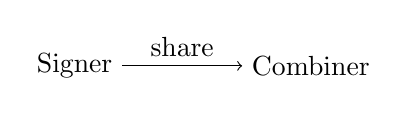
\begin{tikzpicture}
    \node (p) {Signer}; \node (c) at (3,0) {Combiner};
    \draw[->] (p) -- node[above] {share} (c);
  \end{tikzpicture}
  \caption{The two signing rounds.}\label{fig:protocol}
\end{figure}
\input{tables/comparison}
\begin{theorem}\label{thm:unforgeable}
The scheme is unforgeable under the discrete logarithm assumption.
\end{theorem}
